% !TEX root = ../thesis.tex
% !TEX spellcheck = en-US

% doc2vec: highest value is highlighted

% How did I approach the problem, what methods did I evaluate

\clearpage

\section{Results}
\label{sec:Results}

\subsection{Baseline}
\label{sub:Baseline (Results)}

As explained in Section~\ref{sub:Baseline (Experiments)}, uniform and stratified guessing were used as baselines for predictive performance. Averaged over 1000 runs both strategies yielded an \gls{MCC} score close to zero. Accuracy by comparison was around 0.16 for uniform guessing and 0.26 for stratified guessing. These results are to be expected and highlight the reason for choosing \gls{MCC} as the principal metric: \gls{MCC} is zero for random predictions for either strategy whereas the accuracy in the uniform setting corresponds simply to a value of $1/k$ where $k = 6$ is the number of labels. The accuracy in the stratified setting reveals improves by taking advantage of knowledge about the skew in the label distribution. Figure~\ref{fig:guessing-conf-matrix} shows the confusion matrices for these baseline variants in absolute and normalized form, revealing the properties these guessing strategies.

\begin{figure}[h!]
 % From http://localhost:8888/notebooks/thesis/experiments/vector-space-models/Vector%20Space%20Models.ipynb#Baseline:-Guessing-Strategies
    \centering
    \begin{subfigure}[b]{0.47\textwidth}
        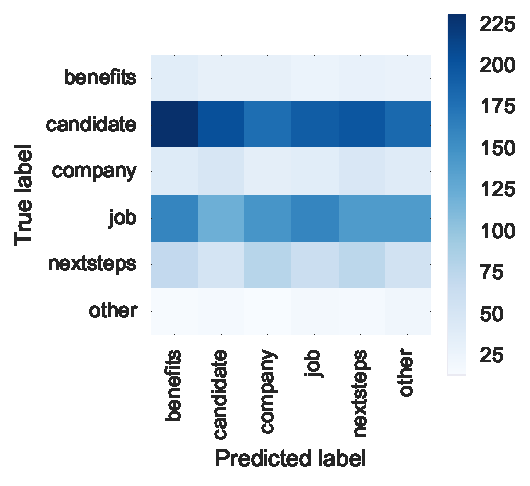
\includegraphics[width=\textwidth]{img/exp-vector-space/guessing-conf-matrix-uniform.pdf}
        \caption{Uniform, absolute}
\label{fig:guessing-conf-matrix-uniform}
    \end{subfigure}
~\begin{subfigure}[b]{0.48\textwidth}
        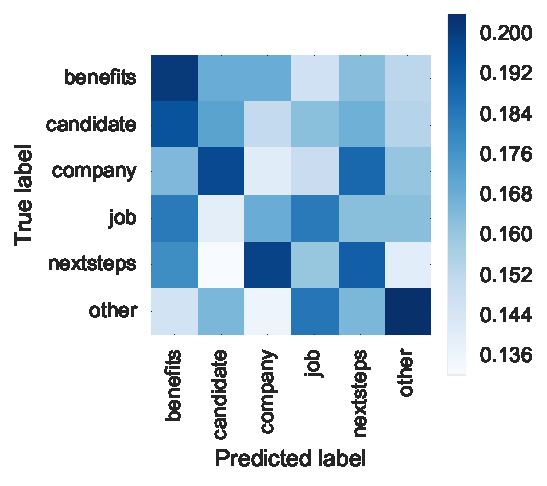
\includegraphics[width=\textwidth]{img/exp-vector-space/guessing-conf-matrix-uniform-normalized.pdf}
        \caption{Uniform, normalized}
\label{fig:guessing-conf-matrix-uniform-normalized}
    \end{subfigure}
~\begin{subfigure}[b]{0.47\textwidth}
        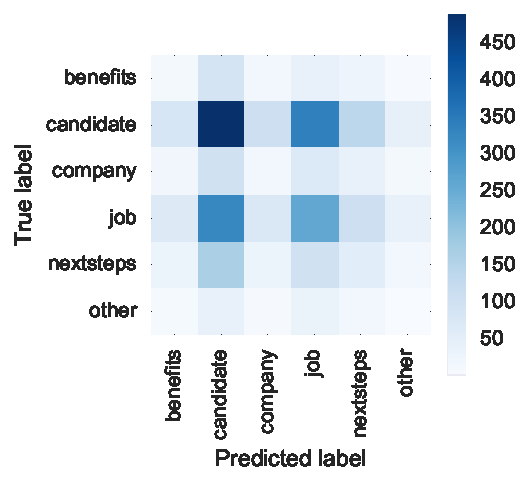
\includegraphics[width=\textwidth]{img/exp-vector-space/guessing-conf-matrix-stratified.pdf}
        \caption{Stratified, absolute}
\label{fig:guessing-conf-matrix-stratified}
    \end{subfigure}
~\begin{subfigure}[b]{0.48\textwidth}
        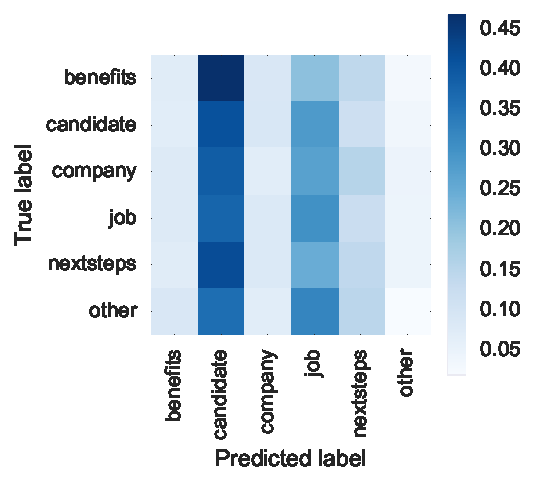
\includegraphics[width=\textwidth]{img/exp-vector-space/guessing-conf-matrix-stratified-normalized.pdf}
        \caption{Stratified, normalized}
\label{fig:guessing-stratified-normalized}
    \end{subfigure}
    \caption{Confusion matrices of uniform and stratified guessing strategies.}
\label{fig:guessing-conf-matrix}
\end{figure}

\clearpage

\subsection{Text Classification Using Vector Space Models}
\label{sub:Text Classification Using Vector Space Models}

\subsubsection{N-gram Models}

\todo{intro here}

\begin{table}[h]
  \begin{center}
  \begin{tabular}{ l l l}
    \toprule
    Hyper-Parameter & N-gram Type: Words & N-gram Type: Characters \\
    \midrule
    N-gram Range (Range) & [1,1], [1,2], [1,3], [2,3], [3,3] & [1,5], [1,10], [5,10], [5,15] \\
    Stop Words & English, None & N/A \\
    Vector Size (Size) & 10, 100, 300 & 10, 100, 300 \\
    IDF & Yes, No & Yes, No \\
    Norm & L1, L2, None & L1, L2, None \\
    Sub-linear TF & Yes, No & Yes, No \\
    \bottomrule
  \end{tabular}
  \caption{Parameter search space word and character level N-gram models}
\label{tab:Ngram Parameters}
\end{center}
\end{table}

The 5 best results of these exhaustive grid searches can be seen in Table~\ref{tab:Ngram Grid Search} below.

\begin{table}[h]
  \begin{center}
  \begin{tabular}{ l l l l l l l l }
    \toprule
    Type & Range & Stop words & Size & IDF & Norm & Sub-linear TF & MCC Score \\
    \midrule
    Word & [1,1] & None & 300 & Yes &  & Yes & 0.689 \\
    Word & [1,1] & None & 300 & Yes &  & No & 0.687 \\
    Word & [1,1] & None & 300 & No &  & Yes & 0.682 \\
    Word & [1,1] & None & 300 & No &  & No & 0.682 \\
    Word & [1,1] & None & 300 & Yes & L2 & Yes & 0.68 \\
    % Word & [1,1] & None & 300 & Yes & L2 & No & 0.678 \\
    % Word & [1,2] & None & 300 & No &  & Yes & 0.677 \\
    % Word & [1,2] & None & 300 & Yes & L2 & Yes & 0.676 \\
    % Word & [1,2] & None & 300 & Yes & L2 & No & 0.675 \\
    % Word & [1,2] & None & 300 & No &  & No & 0.675 \\
    \midrule
    Word & [1,1] & None & 300 & No & & Yes & 0.659  \\
    Word & [1,1] & None & 300 & No & & No & 0.656 \\
    Word & [1,2] & None & 300 & No & & Yes & 0.655 \\
    Word & [1,2] & None & 300 & No & & No & 0.655 \\
    Word & [1,3] & None & 300 & No & & No & 0.65 \\
    % Word & [1,1] & None & 300 & Yes & L2 & Yes & 0.648 \\
    % Word & [1,1] & None & 300 & Yes & L2 & No & 0.648 \\
    % Word & [1,3] & None & 300 & No & & Yes & 0.648 \\
    % Word & [1,2] & None & 300 & Yes & L2 & No & 0.647 \\
    % Word & [1,2] & None & 300 & Yes & L2 & Yes & 0.646 \\
    \midrule
    Word & [1,1] & None & 300 & Yes & & Yes & 0.689 \\
    Word & [1,1] & None & 300 & Yes & & No  & 0.689 \\
    Word & [1,2] & None & 300 & Yes & & Yes & 0.677 \\
    Word & [1,2] & None & 300 & Yes & & No  & 0.677 \\
    Word & [1,3] & None & 300 & Yes & & Yes & 0.674 \\
    % Word & [1,3] & None    & 300 & Yes & & No  & 0.673 \\
    % Word & [1,1] & English & 300 & Yes & & Yes & 0.65 \\
    % Word & [1,1] & English & 300 & Yes & & No  & 0.65 \\
    % Word & [1,2] & English & 300 & Yes & & No  & 0.649 \\
    % Word & [1,2] & English & 300 & Yes & & Yes & 0.648 \\
    \bottomrule
  \end{tabular}
  \caption{Top 5 results of grid search over hyper-parameter space as listed in Table~\ref{tab:Ngram Parameters} using 5-fold cross-validated Logistic Regression (top), Naive Bayes (middle) and SVM (bottom) classifiers.}
\label{tab:Ngram Grid Search}
\end{center}
\end{table}

\todo{Why are the grid scores lower than the latter scores on the train/test split? Because they're averaged and only on the training data?}

Across all classifiers the following results on the hyper-parameters can be observed:

\paragraph{Type}
\label{par:Type}
Words as the atomic unit for N-grams consistently lead to better results. This is understandable as the search space of combinations of characters is significantly larger than the search space of known words.

\paragraph{Range}
\label{par:Range}
There are slight differences to be observed between the three classifiers used, but with all three models the best performance is achieved using Unigrams. Also all of the top results across all classifiers include Unigrams in the model while extending the range towards bigrams or trigrams.

\paragraph{Stop Words}
\label{par:Stop Words}
None of the top results of the performed grid searches used stop words. This is interesting as using stop-words to remove hand-picked, highly frequent words that do not carry much meaning is common practice. It seems there is information carried within these stop words. Of course this outcome is also influenced by the particular stop-list used (see Section~\ref{subp:Stop words}).

\paragraph{Size (matters)}
\label{par:Size}
For the searched settings the largest vector dimensionality of 300 achieves the best performance. This is not surprising as higher-dimensional vectors can capture more information about N-gram occurrences. However in practice the vector size must be limited as it grows with the vocabulary --- potentially at an exponential rate if N-grams other than Unigrams are used. Also very high dimensionality often leads to decreased performance in terms of generalization of the model.

\paragraph{IDF}
\label{par:IDF}
There is no consensus between the classifiers on whether or not to weigh the N-gram frequencies by the \emph{inverse document frequency} (see Section~\ref{subp:TF.IDF weighting}). Thus it seems advisable to lead this parameter free for and evaluate both variants with a given classifier. For logistic regression however the performance differences are marginal and so the choice for this parameter seems somewhat arbitrary.

\paragraph{Norm}
\label{par:Norm}
Is seems that normalizing the vectors in most cases does not lead to any performance gains. Again this is an often recommended practice but here it does not seem to add any value to the model.


\paragraph{Sub-linear TF}
\label{par:Sub-linear TF}
Applying sub-linear TF (see Section~\ref{subp:Sublinear TF scaling}) does not seem to affect the results much and the choice of this parameter can hence be chosen almost arbitrarily as well, although here for all three classifiers applying it leads to a marginal improvement.

Table~\ref{tab:Ngram Grid Search Scores} shows the scores of each classifier using the best N-gram model. It is evident that here logistic regression actually performs best as it offers both, a good accuracy as well as the highest score for Matthews Correlation Coefficient.

\begin{table}[h]
  \begin{center}
  \begin{tabular}{ r | *2l | *2l }
    \toprule
     & \multicolumn{2}{c|}{Training} & \multicolumn{2}{|c}{Validation}\\
    Classifier & Accuracy & MCC & Accuracy & MCC \\
    \midrule
    Logistic Regression & 0.824 & 0.761 & 0.787 & 0.708 \\
    Naive Bayes         & 0.769 & 0.681 & 0.767 & 0.677 \\
    SVM                 & 0.835 & 0.681 & 0.786 & 0.700 \\
    \bottomrule
  \end{tabular}
  \caption{Performance of each best N-gram model with Logistic Regression and Naive Bayes on the validation data}
\label{tab:Ngram Grid Search Scores}
\end{center}
\end{table}

\begin{figure}[h]
    \centering
    \begin{subfigure}[b]{0.32\textwidth}
        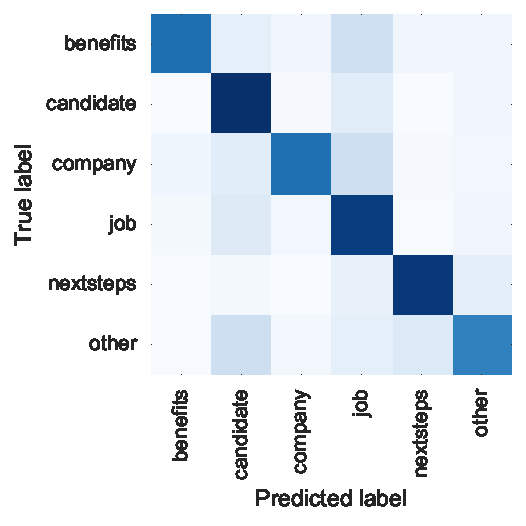
\includegraphics[width=\textwidth]{img/exp-vector-space/ngram-conf-matrix-logreg-normalized.pdf}
        \caption{Logistic Regression}
\label{fig:ngram-conf-matrix-logreg-normalized}
    \end{subfigure}
    \begin{subfigure}[b]{0.32\textwidth}
        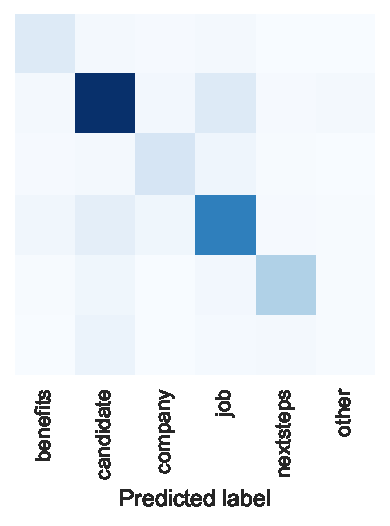
\includegraphics[width=\textwidth]{img/exp-vector-space/ngram-conf-matrix-naivebayes-normalized.pdf}
        \caption{Naive Bayes}
\label{fig:ngram-conf-matrix-naivebayes-normalized}
    \end{subfigure}
    \begin{subfigure}[b]{0.32\textwidth}
        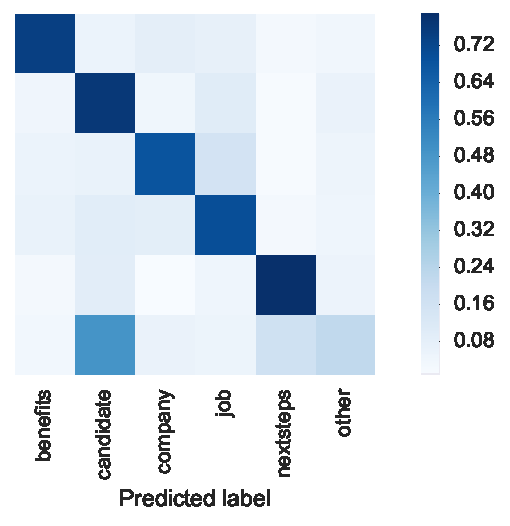
\includegraphics[width=\textwidth]{img/exp-vector-space/ngram-conf-matrix-svm-normalized.pdf}
        \caption{SVM}
\label{fig:ngram-conf-matrix-svm-normalized}
    \end{subfigure}
    \caption{Normalized confusion matrices all three classifiers using the best N-gram model found via cross-validated grid search. Both Naive Bayes as well as SVM show label bias towards the prevalent class \emph{candidate}.}
\label{fig:ngram-conf-matrix}
\end{figure}
\todo{properly align visualization}

Figure~\ref{fig:ngram} shows projections of the of the constructed feature space using the best model that was optimized with Logistic Regression. This visualization shows the separability of the classes in this space. Especially the PCA projection here reveals that it is clearly possible to separate the classes until a certain point.

\begin{figure}[h]
    \centering
    \begin{subfigure}[b]{0.48\textwidth}
      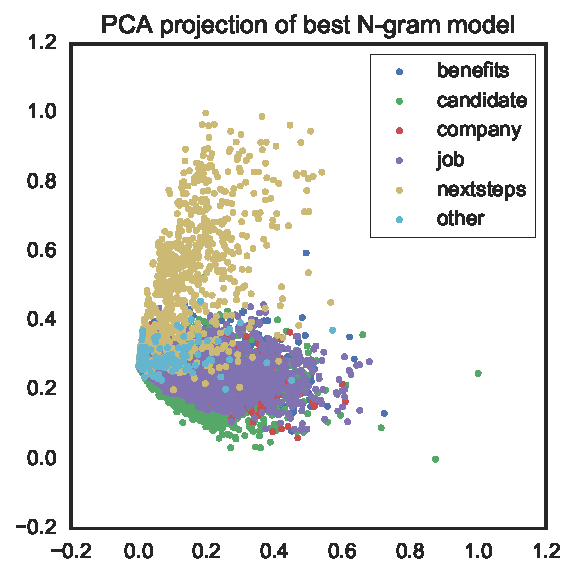
\includegraphics[width=\textwidth]{img/exp-vector-space/ngram-pca.pdf}
      \caption{PCA projection}
\label{fig:ngram-pca}
    \end{subfigure}
~
    %add desired spacing between images, e. g. ~, \quad, \qquad, \hfill etc.
    %(or a blank line to force the subfigure onto a new line)
    \begin{subfigure}[b]{0.48\textwidth}
      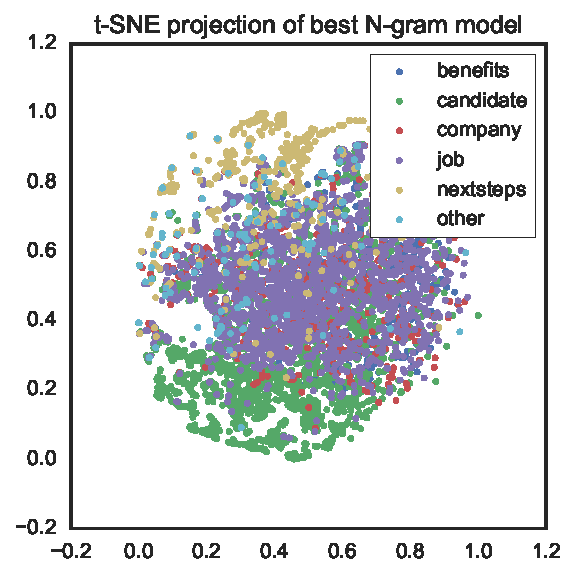
\includegraphics[width=\textwidth]{img/exp-vector-space/ngram-tsne.pdf}
      \caption{t-SNE projection}
\label{fig:ngram-tsne}
    \end{subfigure}
    \caption{Document vectors produced by the best N-gram model (optimized w.r.t. Logistic Regression) projected onto the first 2 principal components (left) and project using t-SNE projection.}
\label{fig:ngram}
\end{figure}

\subsubsection{Bag-of-Means Model}

 The results can be seen in Table~\ref{tab:Bag-Of-Means Results}.

\begin{table}[h]
  \begin{center}
  \begin{tabular}{ r | *2l | *2l }
    \toprule
     & \multicolumn{2}{c|}{Training} & \multicolumn{2}{|c}{Validation}\\
    Classifier & Accuracy & MCC & Accuracy & MCC \\
    \midrule
    Logistic Regression & 0.797 & 0.722 & 0.784 & 0.702 \\
    Naive Bayes         & 0.337 & 0.271 & 0.320 & 0.251 \\
    SVM                 & 0.545 & 0.356 & 0.562 & 0.379 \\
    \bottomrule
  \end{tabular}
  \caption{Performance base classifiers using the Bag-of-Means model}
\label{tab:Bag-Of-Means Results}
\end{center}
\end{table}

The model performs well using Logistic Regression and is almost on par with the best N-gram model. This is surprising as performance previously reported to be rather poor as mention in Section~\ref{subp:Bag-of-Means}. On the other hand the variance in results between the classifiers is huge and especially Naive Bayes seems to perform extremely poor. Further investigation into the use of different classifiers could shed light into these diverging results which are not observed using the N-gram models in the section above. The confusion matrices in Figure~\ref{fig:bom-conf-matrix} reveal strong label bias in the case of Naive Bayes and SVM, although it is unclear where this stems from. Figure~\ref{fig:bom} makes clear though that there is a somewhat meaningful mapping into the feature space. \todo{mention one-vs-all scheme for log reg? also for ngrams above}

\begin{figure}[h]
    \centering
    \begin{subfigure}[b]{0.32\textwidth}
        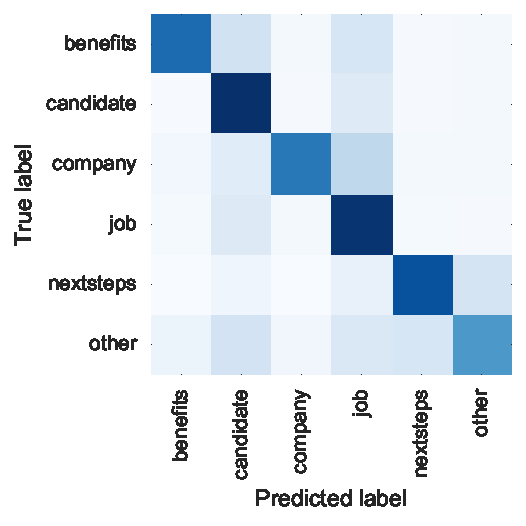
\includegraphics[width=\textwidth]{img/exp-vector-space/bom-conf-matrix-logreg-normalized.pdf}
        \caption{Logistic Regression}
\label{fig:bom-conf-matrix-logreg-normalized}
    \end{subfigure}
    \begin{subfigure}[b]{0.32\textwidth}
        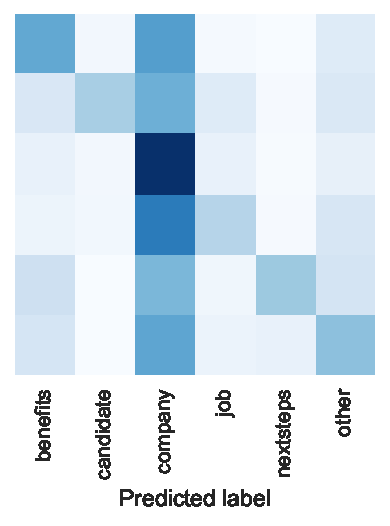
\includegraphics[width=\textwidth]{img/exp-vector-space/bom-conf-matrix-naivebayes-normalized.pdf}
        \caption{Naive Bayes}
\label{fig:bom-conf-matrix-naivebayes-normalized}
    \end{subfigure}
    \begin{subfigure}[b]{0.32\textwidth}
        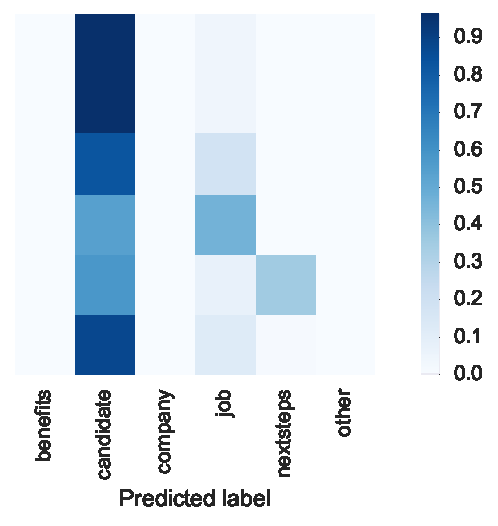
\includegraphics[width=\textwidth]{img/exp-vector-space/bom-conf-matrix-svm-normalized.pdf}
        \caption{SVM}
\label{fig:bom-conf-matrix-svm-normalized}
    \end{subfigure}
    \caption{Normalized confusion matrices of all three classifiers using the Bag-of-Means model.}
\label{fig:bom-conf-matrix}
\end{figure}

\begin{figure}[h]
    \centering
    \begin{subfigure}[b]{0.48\textwidth}
      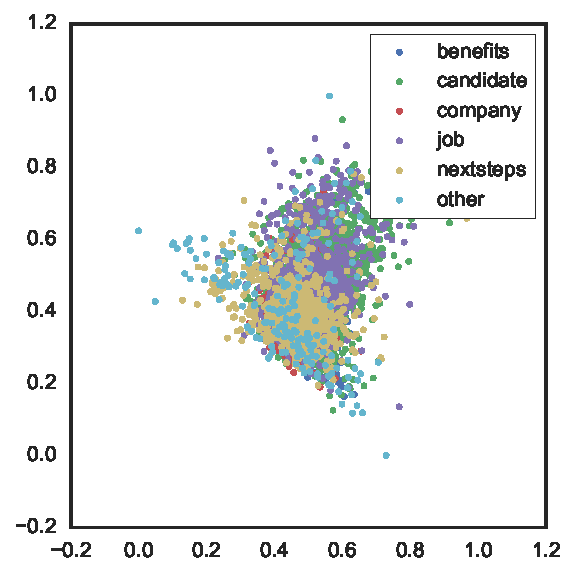
\includegraphics[width=\textwidth]{img/exp-vector-space/bom-pca.pdf}
      \caption{PCA projection}
\label{fig:bom-pca}
    \end{subfigure}
~
    %add desired spacing between images, e. g. ~, \quad, \qquad, \hfill etc.
    %(or a blank line to force the subfigure onto a new line)
    \begin{subfigure}[b]{0.48\textwidth}
      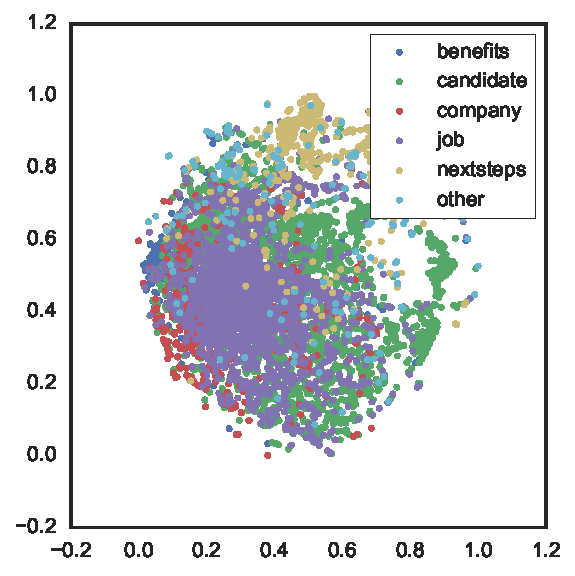
\includegraphics[width=\textwidth]{img/exp-vector-space/bom-tsne.pdf}
      \caption{t-SNE projection}
\label{fig:bom-tsne}
    \end{subfigure}
    \caption{Document vectors produced by Bag-of-Means model (optimized w.r.t. Logistic Regression) projected onto the first 2 principal components (left) and projected using t-SNE projection. It is clear that even though the vectors are simply obtained by averaging they do indeed produce somewhat seperable manifolds.}
\label{fig:bom}
\end{figure}

\subsubsection{Paragraph Vectors using Distributed Representations}


The next sections will briefly outline the results of these tests:\footnote{All tables in this section will use the following abbreviations: \emph{type}: Model Type, i.e. PV-DM vs. PV-DBOW; \emph{size}: Vector Size; \emph{window}: Window Size; \emph{negative}: Negative Sampling value $k$; \emph{hs}: Hierarchical Softmax used; \emph{sample}: Frequent word sub-sampling threshold; \emph{MCC}: Matthews Correlation Coefficient}

\paragraph{Vector Size}
As was to expect the vector size of the model correlates with the performance. Again the highest chosen dimensionality was 300 which yielded the best results with a Matthews Correlation Coefficient of 0.53, however the difference to a 100-dimensional model was marginal with 1\% absolute improvement. Surprisingly even a 10-dimensional vector space model is capable of achieving almost best results with a difference of only 2\% to the 300-dimensional model. Even a 2-dimensional model could achieve a MCC score of 14\%.

\begin{table}[h]
  \begin{center}
    \begin{tabular}{ c | *2c | *2c }
      \toprule
       & \multicolumn{2}{c|}{MCC Training} & \multicolumn{2}{|c}{MCC Test}\\
      Vector Size & Trained & Inferred & Trained & Inferred \\
      \midrule
      2   & 0.302 & 0.255 & 0.173 & 0.251 \\
      10  & 0.457 & 0.417 & 0.296 & \textbf{0.405} \\
      100 & 0.535 & 0.358 & 0.341 & 0.384 \\
      300 & 0.575 & 0.363 & 0.347 & 0.393 \\
      \bottomrule
    \end{tabular}
  \caption{Matthews Correlation Coefficient with varying vector size.}
\label{tab:Paragraph Vector Parameter Results Size}
\end{center}
\end{table}

\begin{figure}[h!]
    \centering
    \begin{subfigure}[b]{0.49\textwidth}
      \includegraphics[width=\textwidth]{img/exp-vector-space/doc2vec_vector_size_2}
      \caption{Vector Size: 2}
\label{fig:doc2vec_vector_size_2}
    \end{subfigure}
    \begin{subfigure}[b]{0.49\textwidth}
      \includegraphics[width=\textwidth]{img/exp-vector-space/doc2vec_vector_size_10}
      \caption{Vector Size: 10}
\label{fig:doc2vec_vector_size_10}
    \end{subfigure}
    \begin{subfigure}[b]{0.49\textwidth}
      \includegraphics[width=\textwidth]{img/exp-vector-space/doc2vec_vector_size_100}
      \caption{Vector Size: 100}
\label{fig:doc2vec_vector_size_100}
  \end{subfigure}
  \begin{subfigure}[b]{0.49\textwidth}
    \includegraphics[width=\textwidth]{img/exp-vector-space/doc2vec_vector_size_300}
    \caption{Vector Size: 300}
\label{fig:doc2vec_vector_size_300}
  \end{subfigure}
\caption{test}
\label{fig:doc2vec_vector_size}
\end{figure}

\paragraph{Frequent Word Sub-Sampling}
Frequent word sub-sampling can boost performance quite much, but again choosing the right value for this hyper-parameter is key. The training behavior with different sampling thresholds differs quite much. Figure~\ref{fig:doc2vec-param-sample} shows the training with different values with 100 passes over the dataset. A good value seems to be $10^{-5}$ which achieves an MCC score of 0.697 and is on-par with the best N-gram model. Interestingly not using sub-sampling in this setup seemed to be overfitting as the score decreases quite drastically with more training passes. A similar effect is observed with a higher threshold of $10^{-4}$ but much less strong. Choosing a lower threshold of $10^{-6}$ leads to very poor performance with an MCC score of only 0.07.

\begin{table}[h]
  \begin{center}
    \begin{tabular}{ c | *2c | *2c }
      \toprule
       & \multicolumn{2}{c|}{MCC Training} & \multicolumn{2}{|c}{MCC Test}\\
      Sub-sampling threshold & Trained & Inferred & Trained & Inferred \\
      \midrule
      No sub-sampling & 0.536 & 0.363 & 0.336 & 0.384 \\
      1e-4 & 0.627 & 0.377 & 0.315 & \textbf{0.397} \\
      1e-5 & 0.599 & 0.250 & 0.173 & 0.247 \\
      1e-6 & 0.431 & 0.147 & 0.106 & 0.129 \\
    \bottomrule
  \end{tabular}
  \caption{Matthews Correlation Coefficient with varying frequent word sub-sampling threshold.}
\label{tab:Paragraph Vector Parameter Results Sample}
\end{center}
\end{table}

\begin{figure}[h!]
    \centering
    \begin{subfigure}[b]{0.49\textwidth}
      \includegraphics[width=\textwidth]{img/exp-vector-space/doc2vec_sample_0}
      \caption{No Sub-Sampling}
\label{fig:doc2vec_sample_0}
    \end{subfigure}
    \begin{subfigure}[b]{0.49\textwidth}
      \includegraphics[width=\textwidth]{img/exp-vector-space/doc2vec_sample_1e-4}
    \caption{Sub-Sampling Threshold: 1e-4}
\label{fig:doc2vec_vector_size_1e-4}
    \end{subfigure}
    \begin{subfigure}[b]{0.49\textwidth}
      \includegraphics[width=\textwidth]{img/exp-vector-space/doc2vec_sample_1e-5}
      \caption{Sub-Sampling Threshold: 1e-5}
\label{fig:doc2vec_vector_size_1e-5}
  \end{subfigure}
  \begin{subfigure}[b]{0.49\textwidth}
    \includegraphics[width=\textwidth]{img/exp-vector-space/doc2vec_sample_1e-6}
    \caption{Sub-Sampling Threshold: 1e-6}
\label{fig:doc2vec_sample_1e-6}
  \end{subfigure}
\caption{test}
\label{fig:doc2vec_sample}
\end{figure}

\paragraph{Hierarchical Softmax}
Using hierarchical softmax increased the performance, leading to a 12\% absolute difference in terms of MCC score. This result is counter-intuitive as using the hierarchical softmax should as an approximation be less performant. However it might simply mitigate overfitting of the model.

\begin{table}[h]
  \begin{center}
    \begin{tabular}{ c | *2c | *2c }
      \toprule
       & \multicolumn{2}{c|}{MCC Training} & \multicolumn{2}{|c}{MCC Test}\\
      Hierarchical Softmax & Trained & Inferred & Trained & Inferred \\
      \midrule
      Not used & 0.364 & 0.195 & 0.201 & 0.236 \\
      Used     & 0.534 & 0.365 & 0.340 & \textbf{0.387} \\
    \bottomrule
  \end{tabular}
  \caption{Matthews Correlation Coefficient with and without using hierarchical softmax.}
\label{tab:Paragraph Vector Parameter Results Hierarchical Softmax}
\end{center}
\end{table}

\begin{figure}[h!]
    \centering
    \begin{subfigure}[b]{0.49\textwidth}
      \includegraphics[width=\textwidth]{img/exp-vector-space/doc2vec_hs_0}
      \caption{Without Hierarchical Softmax}
\label{fig:doc2vec_hs_0}
    \end{subfigure}
    \begin{subfigure}[b]{0.49\textwidth}
      \includegraphics[width=\textwidth]{img/exp-vector-space/doc2vec_hs_1}
    \caption{With Hierarchical Softmax}
\label{fig:doc2vec_hs_1}
    \end{subfigure}
\caption{test}
\label{fig:doc2vec_hs}
\end{figure}

\paragraph{Negative Sampling}
Negative Sampling generally increased the performance of the model and smaller values actually worked best out of the tested settings from 0 to 6. Choosing the number of negative samples to be 2 resulted in the best performance, but the absolute difference in performance was only about 6\% of achieved MMC score.

\begin{table}[h]
  \begin{center}
    \begin{tabular}{ c | *2c | *2c }
      \toprule
       & \multicolumn{2}{c|}{MCC Training} & \multicolumn{2}{|c}{MCC Test}\\
      Negative Sampling Value & Trained & Inferred & Trained & Inferred \\
      \midrule
      0 & 0.581 & 0.221 & 0.332 & 0.343 \\
      2 & 0.555 & 0.338 & 0.363 & \textbf{0.399} \\
      4 & 0.517 & 0.336 & 0.350 & 0.378 \\
      6 & 0.489 & 0.317 & 0.338 & 0.363 \\
    \bottomrule
  \end{tabular}
  \caption{Matthews Correlation Coefficient with varying negative sampling value.}
\label{tab:Paragraph Vector Parameter Results Negative Sampling}
\end{center}

\end{table}

\begin{figure}[h!]
    \centering
    \begin{subfigure}[b]{0.49\textwidth}
      \includegraphics[width=\textwidth]{img/exp-vector-space/doc2vec_negative_0}
      \caption{Negative Sampling Value: 2}
\label{fig:doc2vec_negative_0}
    \end{subfigure}
    \begin{subfigure}[b]{0.49\textwidth}
      \includegraphics[width=\textwidth]{img/exp-vector-space/doc2vec_negative_2}
    \caption{Negative Sampling Value: 2}
\label{fig:doc2vec_vector_size_2}
    \end{subfigure}
    \begin{subfigure}[b]{0.49\textwidth}
      \includegraphics[width=\textwidth]{img/exp-vector-space/doc2vec_negative_4}
      \caption{Negative Sampling Value: 4}
\label{fig:doc2vec_vector_size_4}
  \end{subfigure}
  \begin{subfigure}[b]{0.49\textwidth}
    \includegraphics[width=\textwidth]{img/exp-vector-space/doc2vec_negative_6}
    \caption{Negative Sampling Value: 6}
\label{fig:doc2vec_negative_6}
  \end{subfigure}
\caption{test}
\label{fig:doc2vec_negative}
\end{figure}

\paragraph{Window Size}
Window sizes of 5, 10 and 15 were experimented with which increase or decrease the width of context the model is trained on. Here a window size of 10 showed best results. It is safe to assume that increasing the window size much further does not lead to any improvement in the model as the correlation with the word should become weaker the farther we move away from it in a document or text.

\begin{table}[h]
  \begin{center}
    \begin{tabular}{ c | *2c | *2c }
      \toprule
       & \multicolumn{2}{c|}{MCC Training} & \multicolumn{2}{|c}{MCC Test}\\
      Window size & Trained & Inferred & Trained & Inferred \\
      \midrule
      5 & 0.534 & 0.358 & 0.380 & \textbf{0.411} \\
      10 & 0.540 & 0.347 & 0.366 & 0.393 \\
      15 & 0.536 & 0.317 & 0.339 & 0.373 \\
    \bottomrule
    \end{tabular}
  \caption{Matthews Correlation Coefficient with varying window size.}
\label{tab:Paragraph Vector Parameter Results Window Size}
\end{center}
\end{table}

\begin{figure}[h!]
    \centering
    \begin{subfigure}[b]{0.49\textwidth}
      \includegraphics[width=\textwidth]{img/exp-vector-space/doc2vec_window_5}
      \caption{Window Size: 5}
\label{fig:doc2vec_window_5}
    \end{subfigure}
    \begin{subfigure}[b]{0.49\textwidth}
      \includegraphics[width=\textwidth]{img/exp-vector-space/doc2vec_window_10}
    \caption{Window Size: 10}
\label{fig:doc2vec_window_10}
    \end{subfigure}
    \begin{subfigure}[b]{0.49\textwidth}
      \includegraphics[width=\textwidth]{img/exp-vector-space/doc2vec_window_15}
      \caption{Window Size: 15}
\label{fig:doc2vec_window_15}
  \end{subfigure}
\caption{test}
\label{fig:window}
\end{figure}


\paragraph{PV-DBOW versus PM-DV}
Both models for paragraph vectors proposed in~\cite{Le:2014aa} were tried, namely Distributed Bag of Words version of Paragraph Vector (PV-DBOW) and Distributed Memory version of Paragraph Vector (PV-DM). In these tests the DBOW model achieves significantly better results with an MCC that is 14\% than the PV-DM model in absolute terms. This is in contrast with the results in the aforementioned paper, where the authors state that \textquote{PV-DM is consistently better than PV-DBOW.}~\cite{Le:2014aa}.

\begin{table}[h]
  \begin{center}
    \begin{tabular}{ c | *2c | *2c }
      \toprule
       & \multicolumn{2}{c|}{MCC Training} & \multicolumn{2}{|c}{MCC Test}\\
      Window size & Trained & Inferred & Trained & Inferred \\
      \midrule
      PV-BBOW & 0.627 & 0.610 & 0.544 & \textbf{0.582} \\
      PV-DM   & 0.534 & 0.365 & 0.341 & 0.391 \\
    \bottomrule
    \end{tabular}
    \caption{Matthews Correlation Coefficient using the two models proposed in~\cite{Le:2014aa}.}
\label{tab:Paragraph Vector Parameter Results PV-DBOW versus PM-DV}
\end{center}
\end{table}

\begin{figure}[h!]
    \centering
    \begin{subfigure}[b]{0.49\textwidth}
      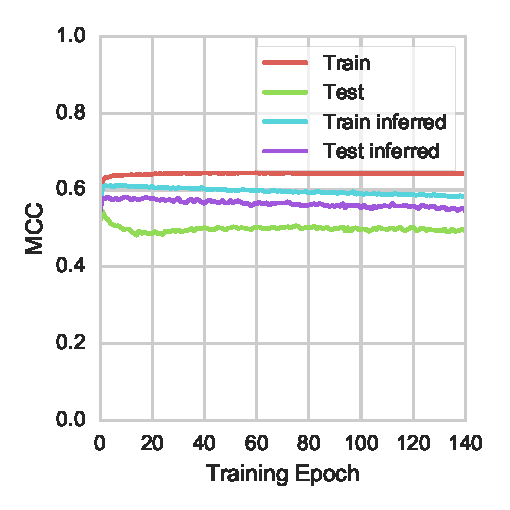
\includegraphics[width=\textwidth]{img/exp-vector-space/doc2vec_dm_0}
      \caption{PV-DBOW Model}
\label{fig:doc2vec_dm_0}
    \end{subfigure}
    \begin{subfigure}[b]{0.49\textwidth}
      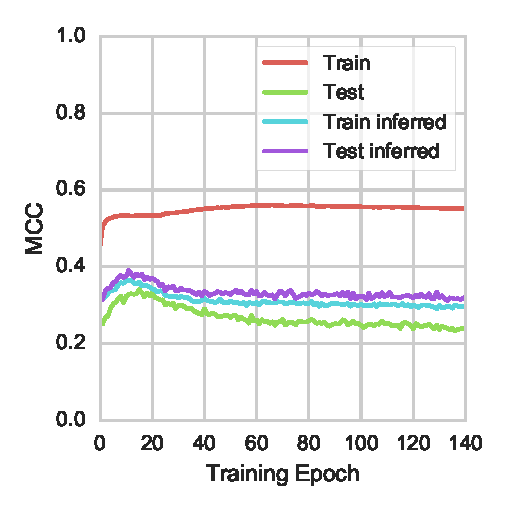
\includegraphics[width=\textwidth]{img/exp-vector-space/doc2vec_dm_1}
    \caption{PV-DM Model}
\label{fig:doc2vec_dm_1}
    \end{subfigure}
  \caption{test}
\label{fig:doc2vec_doc2vec_dm}
\end{figure}

\todo{show computation time?}

\paragraph{Evaluating the best hyper-parameter setting}

Taking the learnings about the effects of the different hyper-parameters to the performance of the model a subset of models were tested in search of the best hyper-parameter selection. The results of these experiments can be seen in Table~\ref{tab:Paragraph Vector Parameter Results Best}.

A few interesting observations can be made here. First, as indicated before, the model is highly sensitive to the settings of the hyper-parameters. Secondly we can see that the hyper-parameters interact quite strongly in some combinations. This leads to a different behavior in performance for some of the hyper-parameters than identified in the above sections, depending on what the other hyper-parameters settings are.

For instance using hierarchical softmax decreases performance when setting all other parameters to individually optimal settings, as opposed to in the previous experiment above.
\todo{write a bit more here}

\begin{table}[h]
  \begin{center}
  \begin{tabular}{ *6l | l }
    \toprule
    type & size & window & negative & hs & sample & MCC  \\
    \midrule
    PV-DM & 300 & 10 & 3 & 0 & 1e-5 & 0.707 \\
    PV-BBOW & 300 & 10 & 3 & 0 & 1e-5 & 0.724 \\
    PV-BBOW & 300 & 10 & 3 & 1 & 1e-5 & 0.665 \\
    \bottomrule
  \end{tabular}
  \caption{Matthews Correlation Coefficient of different models when trying to find the best hyper-parameter setting.}
\label{tab:Paragraph Vector Parameter Results Best}
\end{center}
\end{table}


% \subsubsection{Paragraph Vectors using pre-initialized weights *}
%
% In another experiment the weight matrix for the words was initialized with pre-trained weights from from the Google News dataset.

% \subsubsection{Paragraph Vectors using context sentences *}
%
% \todo{This section in further research? Because it would have to be done for N-grams as well (building a model with the context around a sentence) and it doesn't fit the task (only sentence given). Could also go into exploration}

% \subsubsection{Inversion of Distributed Language Representations (??)}
%
% \todo{if this is described here it has to go into background as well}

% \subsubsection{Discussion *}


\subsubsection{Classification Methods Using Vector Space Models}
\label{subs:subsection label}

\paragraph{Logistic Regression}
\paragraph{Decision Tree}
\paragraph{Naive Bayes}
\paragraph{SVM}
\paragraph{KNN}
\paragraph{Random Forest}
\paragraph{Neural Network}
\paragraph{Deep Neural Network}
\paragraph{Convolutional Neural Network}

\subsection{Sequential Text Classification}

\subsubsection{Character-based LSTM *}

\subsubsection{Character-based Multi-task LSTM *}

\subsection{Comparison of Approaches}
